\chapter{Methodology}
\label{chapter:methodology}

This chapter describes the methodology proposed to assess prosthetic
adaptation from the data acquired by the instrumented prosthesis. Rather than
committing prematurely to a specific learning algorithm, the methodology is
organised around a \emph{data pipeline}: a sequence of well-defined processing
stages that transforms raw sensor signals into an interpretable adaptation
estimate. The classification model itself is the final, and largely
interchangeable, stage of this pipeline; the central methodological
contribution lies in how the signals are processed, which features are
extracted, and how adaptation is defined and labelled.

\section{Data Processing Pipeline}
\label{section:pipeline}

The proposed approach does not feed the raw inertial and force signals directly
into a model. Instead, it extracts a compact set of interpretable biomechanical
features and uses these as the model input. This design decision is motivated by
two constraints inherent to the application: the dataset is small and acquired
incrementally, and the resulting assessment must be interpretable in a clinical
context~\cite{Mannini2016}. End-to-end approaches that learn directly
from raw signals are powerful but require large labelled datasets and yield
limited interpretability; they are therefore identified as a direction for
future work once a sufficiently large multi-subject dataset becomes available.

Figure~\ref{fig:pipeline} summarises the complete pipeline, from raw
acquisition to the adaptation estimate.

\begin{figure}[ht]
  \centering
  \begin{tikzpicture}[
      node distance=6mm,
      stage/.style={
        draw, rounded corners, align=center, text width=8.2cm,
        minimum height=9mm, font=\small, fill=blue!5},
      lbl/.style={font=\scriptsize\itshape, text=black!60},
      arr/.style={-{Latex[length=2.5mm]}, thick}
    ]
    \node[stage] (acq)  {\textbf{1. Acquisition} --- raw CSV at 80\,Hz \\
                          (IMU 9-axis, load cell, orientation)};
    \node[stage, below=of acq] (seg) {\textbf{2. Stride segmentation} ---
                          split continuous signal into gait cycles};
    \node[stage, below=of seg] (feat) {\textbf{3. Feature extraction} ---
                          force, temporal and variability metrics};
    \node[stage, below=of feat] (agg) {\textbf{4. Aggregation} ---
                          summarise features per run/session};
    \node[stage, below=of agg] (model) {\textbf{5. Classification model} ---
                          features $\rightarrow$ adaptation state};
    \node[stage, below=of model] (out) {\textbf{6. Output} ---
                          adaptation score (binary or continuous)};

    \draw[arr] (acq)   -- (seg);
    \draw[arr] (seg)   -- (feat);
    \draw[arr] (feat)  -- (agg);
    \draw[arr] (agg)   -- (model);
    \draw[arr] (model) -- (out);

    \node[lbl, right=2mm of acq.east]  {already implemented};
    \node[lbl, right=2mm of feat.east] {core contribution};
  \end{tikzpicture}
  \caption{Proposed data processing pipeline. Stage~1 is already implemented in
           the current prototype; the methodological core of this work lies in
           the stride segmentation and feature extraction stages (2--4), while
           the classification model (5) is treated as an interchangeable final
           component.}
  \label{fig:pipeline}
\end{figure}

The acquisition stage already exists in the current prototype: data is acquired
at 80\,Hz, as justified in Chapter~\ref{chapter:proposed}, and written directly
as clean session files. The remaining stages constitute the methodological work
proposed for this thesis and are detailed below.

\section{Stride Segmentation}
\label{section:segmentation}

All subsequent metrics depend on partitioning the continuous recording into
individual gait cycles. Two complementary and redundant detectors are used to
improve robustness. The load-cell signal exhibits distinct periodic peaks
corresponding to ground-contact events, while the vertical acceleration
captures the characteristic stance-phase profile. Foot-strike and toe-off
events are identified by peak detection on the force signal, cross-validated
against the vertical-acceleration profile, with a minimum inter-event distance
derived from the expected canine stride frequency of
2--4\,Hz~\cite{Jenkins2018,Hayati2019}. This segmentation yields the temporal
boundaries of stance and swing phases for each stride.

\section{Biomechanical Features}
\label{section:features}

From each segmented stride, a set of interpretable features is extracted,
organised into four groups that together provide a compact representation of
locomotor behaviour while remaining computationally lightweight enough for
resource-constrained processing~\cite{Preece2009,Bulling2014}. The first two
groups exploit the two sensing modalities directly --- \emph{kinetic} features
from the load cell and \emph{kinematic} features from the IMU --- while the
\emph{temporal} and \emph{variability} groups summarise the timing and the
step-to-step consistency of the movement.
Figure~\ref{fig:gait_cycle} illustrates the force-based features schematically on
a single gait cycle, defining the phases and quantities referred to throughout
this section.

\begin{figure}[ht]
  \centering
  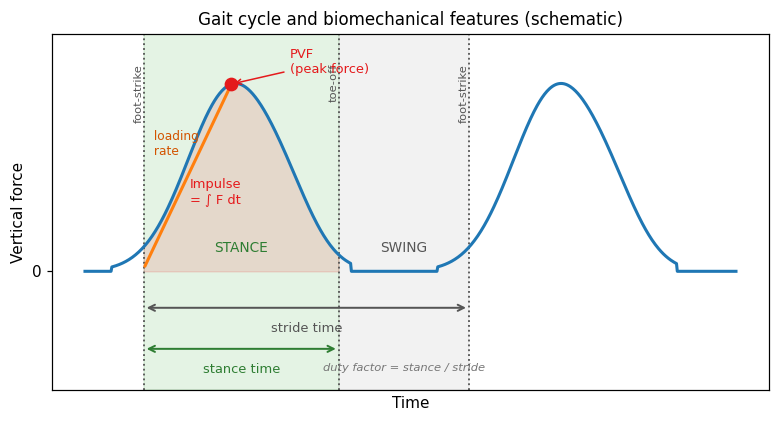
\includegraphics[width=0.85\linewidth]{05_figures/05_methodology/feat_gait_cycle}
  \caption{Schematic of a single gait cycle measured by the prosthetic load
           cell, annotated with the biomechanical features. The stance phase
           (foot-strike to toe-off) carries the load: its peak is the peak
           vertical force (PVF), the shaded area is the vertical impulse, and
           the initial slope is the loading rate. The stride spans consecutive
           foot-strikes, and the duty factor is the stance-to-stride ratio.}
  \label{fig:gait_cycle}
\end{figure}

\paragraph{Kinetic features (load cell).}
These features describe how the prosthetic limb accepts and transmits load, and
are the most direct evidence of whether the animal is willing to bear weight on
the prosthesis~\cite{Oosterlinck2011,Fahie2018}.

\paragraph{Kinematic features (IMU).}
Derived from the inertial unit, these features describe how the prosthesis moves
through space: the angular excursion (range of motion) of the limb, the vigour
of the swing, and the smoothness of the movement. Movement smoothness is a
particularly informative adaptation marker, as motor learning is accompanied by
a transition from rigid, guarded movement towards smoother, better-coordinated
patterns~\cite{Wurdeman2014,Mannini2016}.

\paragraph{Temporal features.}
Derived from the segmented gait cycles, these features describe the timing
structure of locomotion and characterise the rhythm and phase organisation of
each stride~\cite{Jenkins2018,Zhang2022}.

\paragraph{Variability features.}
Computed across consecutive strides rather than within a single stride, these
features are central to the single-limb adaptation assessment, as reduced
stride-to-stride variability is associated with improved adaptation to a
prosthesis~\cite{Wurdeman2014,Blattler2024}.

Table~\ref{tab:features} details the individual features of each group, together
with the aspect of locomotion that each is intended to assess.
Figures~\ref{fig:feat_force},~\ref{fig:feat_var} and~\ref{fig:feat_kin} show
these features computed on a real walking session, confirming that the schematic
of Figure~\ref{fig:gait_cycle} is recovered from the acquired signals and that
the IMU contributes complementary kinematic information.

\begin{table}[ht]
  \centering
  \caption{Biomechanical features extracted per stride and the aspect of
           prosthetic use each one assesses.}
  \label{tab:features}
  \small
  \begin{tabular}{p{3.1cm} p{4.0cm} p{5.0cm}}
    \toprule
    \textbf{Feature} & \textbf{Definition} & \textbf{What it assesses} \\
    \midrule
    \multicolumn{3}{l}{\textit{Kinetic (load cell)}} \\
    \midrule
    Peak vertical force (PVF)
      & Maximum axial force during the stance phase
      & How much weight the animal places on the prosthesis; low values
        indicate the limb is being spared \\
    Vertical impulse
      & Integral of force over the stance phase
      & Total load transmitted per step, combining force magnitude and
        contact duration \\
    Loading rate
      & Slope of the force rise at ground contact
      & How confidently and abruptly the limb is loaded; hesitant loading
        suggests discomfort or distrust of the prosthesis \\
    Weight-bearing ratio
      & Fraction of strides with full ground contact
      & Consistency of prosthesis use; frequent light or missing contacts
        indicate avoidance \\
    \midrule
    \multicolumn{3}{l}{\textit{Kinematic (IMU)}} \\
    \midrule
    Pitch / roll range of motion
      & Angular excursion of the limb within each stride
      & Amplitude of limb movement; a reduced range reflects guarded, stiff
        use of the prosthesis \\
    Peak angular rate
      & Maximum resultant gyroscope magnitude per stride
      & Vigour and speed of the swing phase \\
    Limb angle at peak force
      & Pitch at the instant of PVF
      & Consistency of limb placement at the moment of loading \\
    Movement smoothness (SPARC)
      & Spectral arc length of the angular-rate profile
      & Motor coordination; smoother (less jerky) movement is associated with
        better adaptation \\
    \midrule
    \multicolumn{3}{l}{\textit{Temporal (gait segmentation)}} \\
    \midrule
    Stride time
      & Duration of one complete gait cycle
      & Overall gait pace and its regularity over the session \\
    Stance / swing time
      & Duration of the ground-contact and aerial phases
      & Whether the limb completes a normal load-bearing phase or is lifted
        prematurely \\
    Duty factor
      & Ratio of stance time to stride time
      & Proportion of the cycle spent bearing load; a shortened stance
        reflects guarded use of the prosthesis \\
    Cadence
      & Number of strides per unit time
      & Locomotor rhythm and willingness to move at a normal pace \\
    \midrule
    \multicolumn{3}{l}{\textit{Variability (across consecutive strides)}} \\
    \midrule
    CV of stride time
      & Coefficient of variation of stride duration
      & Temporal consistency of gait; high variability reflects an unstable,
        poorly adapted pattern \\
    CV of peak force
      & Coefficient of variation of PVF
      & Consistency of load acceptance from step to step \\
    Stride-to-stride autocorrelation
      & Self-similarity of consecutive force/acceleration cycles
      & Periodicity and repeatability of the gait pattern; higher regularity
        indicates better adaptation \\
    CV of kinematic features
      & Coefficient of variation of pitch range of motion and peak angular rate
      & Consistency of the movement pattern itself, complementing the
        force-based variability \\
    \bottomrule
  \end{tabular}
\end{table}

\begin{figure}[ht]
  \centering
  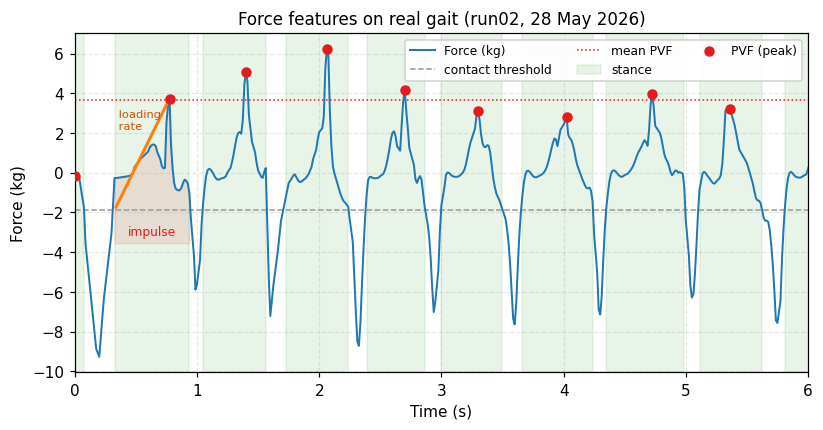
\includegraphics[width=0.92\linewidth]{05_figures/05_methodology/feat_force_real}
  \caption{Force-related features extracted from a real walking session.
           Detected stance phases are shaded, the contact threshold and mean
           PVF are marked, and the per-stride peaks (PVF) are highlighted; one
           stride additionally shows the vertical impulse (shaded area) and the
           loading-rate slope.}
  \label{fig:feat_force}
\end{figure}

\begin{figure}[ht]
  \centering
  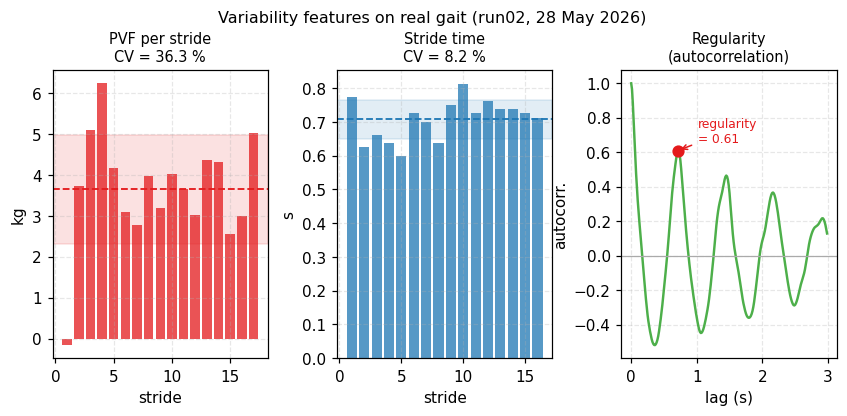
\includegraphics[width=0.98\linewidth]{05_figures/05_methodology/feat_variability_real}
  \caption{Variability features from the same session. Left and centre: peak
           vertical force and stride time per stride, with the mean (dashed)
           and $\pm$one standard deviation band; the coefficient of variation
           (CV) summarises each. Right: the autocorrelation of the force signal,
           whose first dominant peak gives the regularity index (higher values
           indicate a more periodic, repeatable gait).}
  \label{fig:feat_var}
\end{figure}

\begin{figure}[ht]
  \centering
  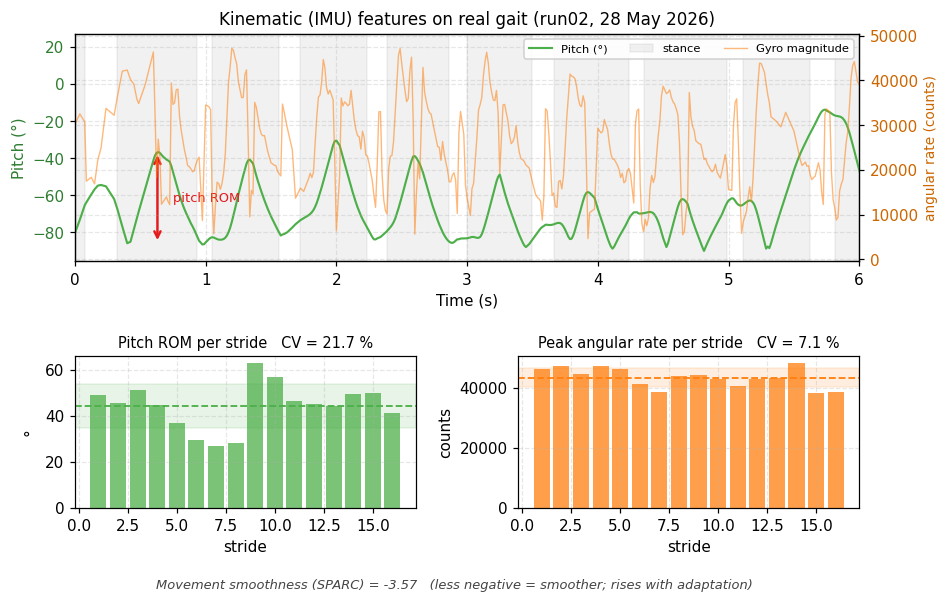
\includegraphics[width=0.95\linewidth]{05_figures/05_methodology/feat_kinematic_real}
  \caption{Kinematic features from the IMU on the same session. Top: limb pitch
           (green) and gyroscope magnitude (orange) with stance phases shaded;
           the pitch range of motion is annotated on one stride. Bottom: pitch
           range of motion and peak angular rate per stride, with their
           coefficients of variation; the overall movement smoothness (SPARC) is
           reported below. Together these capture how the prosthesis moves, in
           complement to the force-based features.}
  \label{fig:feat_kin}
\end{figure}

\section{Adaptation Assessment and Labelling Strategy}
\label{section:adaptation}

Because only the prosthetic limb is instrumented, the inter-limb symmetry
metrics commonly used in gait analysis are not
applicable~\cite{Oosterlinck2011,Fahie2018}. Adaptation is therefore assessed
through the \emph{longitudinal consistency and stability} of the extracted
features: a well-adapted prosthesis is expected to produce consistent load
patterns, regular timing, smooth limb motion, and low stride-to-stride
variability, whereas poor adaptation manifests as irregular loading, jerky
movement, and increased variability.

Supervised learning requires a ground-truth label for the adaptation state, and
defining this label is a central methodological challenge. The proposed
strategy combines two complementary sources:

\paragraph{Clinical scoring (primary label).}
Each acquisition session is rated by the veterinary team of the partner
hospital using a simple ordinal scale (for example, a 0--4 score of prosthesis
use, comfort, or limb loading). This expert assessment constitutes the primary
ground truth. Crucially, because the label is assigned \emph{per session}, no
fine-grained temporal synchronisation between the sensor stream and the
assessment is required: each recording carries an NTP-synchronised timestamp
that unambiguously associates it with the corresponding clinical evaluation.

\paragraph{Temporal progression (validation signal).}
For a given subject, adaptation is expected to improve gradually across
sessions~\cite{Rosen2022,Wendland2019}. The temporal ordering of sessions is
therefore used not as the primary label but as an independent consistency check
on the clinical scores and on the extracted features.

\paragraph{Role of video.}
Video is recorded during a subset of sessions and serves two auxiliary
purposes. First, it validates the stride-segmentation stage: a deliberate
alignment event at the start of a run (e.g.\ tapping the prosthesis) produces a
signature visible in both the signal and the video, allowing the detected
force peaks to be confirmed against actual foot contacts. Second, it allows the
clinical score to be assigned from recorded footage rather than in real time,
improving the reliability and repeatability of the labels. Video is thus an
instrument for validation and label refinement, not a requirement for the core
classification.

\section{Machine Learning Formulation}
\label{section:ml}

The assessment of prosthetic adaptation is formulated as a supervised
classification problem mapping the vector of biomechanical features to an
adaptation state. The output may be defined as a binary classification
(adapted vs.\ non-adapted) or as a multi-level scale representing degrees of
adaptation.

The methodology deliberately does not fix a single algorithm in advance.
Tree-based ensembles, particularly Random Forest, are a suitable starting point
due to their robustness to noise, ability to model non-linear relationships,
strong performance on small datasets, and the interpretability afforded by
feature-importance analysis~\cite{Bulling2014,Wang2019}. Simpler baselines such
as logistic regression and support vector machines will also be
evaluated~\cite{Mannini2016}. The final model will be selected on the basis of
classification performance and interpretability once sufficient data are
available. The pipeline of Figure~\ref{fig:pipeline} is intentionally agnostic
to this choice.

As an alternative for the regime in which clinical labels are scarce or
unavailable, unsupervised and one-class methods (e.g.\ isolation forests or
one-class support vector machines) will be considered: a model is trained on
stable locomotion and the deviation of new data from this learned
``normal'' is interpreted as a degree of mal-adaptation~\cite{Otamendi2023}.
This provides a fallback that requires no labelled data and complements the
supervised formulation.

\section{Evaluation Plan}
\label{section:evaluation}

Evaluation has both a longitudinal and a classification component. The
longitudinal analysis compares locomotion patterns across multiple sessions of
the same subject, examining intra-subject variability and the progression of
the extracted features as indicators of improvement or degradation in
prosthesis use~\cite{Rosen2022,Wendland2019}. The classification model is
assessed using standard metrics (accuracy, precision, recall) and, critically,
a subject-aware validation scheme. Because consecutive strides of the same
animal are strongly correlated, random data splits would leak information and
overestimate performance; a \emph{leave-one-subject-out} cross-validation will
therefore be adopted once data from multiple dogs are available. Where the
output is continuous, the gradual evolution of the adaptation estimate can be
related to motor-learning models, in which adaptation typically follows an
exponential progression towards a stable asymptote~\cite{Reinkensmeyer2016}.

\section{Open Questions}
\label{section:open_questions}

As an initial proposal, several aspects are intentionally left to be specified
during the experimental phase, and are stated here explicitly:
\begin{itemize}
  \item the exact definition and granularity of the clinical scoring scale,
        to be agreed with the veterinary team;
  \item the number of canine subjects and sessions in the acquisition
        campaign, which determines the feasibility of supervised versus
        unsupervised formulations;
  \item the video acquisition protocol (camera placement, alignment event,
        and the subset of sessions to be filmed).
\end{itemize}
Specifying these decisions is part of the planned work and does not affect the
overall structure of the proposed pipeline.
